\section{方程与初值}
\label{sec:ivp-equations}

一条未知曲线怎样被“变化规律”和“起点”确定下来？先看两个增长的例子，再看冷却，然后把共同的结构写成定义。

\paragraph{指数增长}
设$x(t)$是培养液中细菌的数量（以某个单位计），$t$是时间。营养充足时，每个细菌在单位时间内分裂的机会相同，所以单位时间的增量与现有数量成正比，比例系数记作$r>0$：
\begin{equation}
 \dot{x}(t)=r\,x(t).
 \label{eq:ivp-exponential}
\end{equation}
字母上方的点表示对时间$t$求导，$\dot{x}(t)=\mathrm{d}x/\mathrm{d}t$，两个点表示二阶导数$\ddot{x}$。式~\eqref{eq:ivp-exponential}没有告诉我们$x(t)$是多少，只告诉我们每个时刻曲线的斜率与当时的高度之比是$r$。

我们知道指数函数的导数还是它自己乘以系数，所以对任意常数$C$，曲线$x(t)=C\mathrm{e}^{rt}$都满足式~\eqref{eq:ivp-exponential}。一条规律对应一族曲线。要从中选出一条，需要再说明某个时刻的数量。若$t=0$时数量为$x_0$，代入得$C=x_0$，于是
\begin{equation}
 x(t)=x_0\mathrm{e}^{rt}.
 \label{eq:ivp-exponential-solution}
\end{equation}

\paragraph{饱和增长}
营养有限时，数量越接近培养液能养活的上限$K$，每个细菌分裂得越慢。最简单的写法是把比例系数$r$改成$r(1-x/K)$：
\begin{equation}
 \dot{x}=r\,x\Bigl(1-\frac{x}{K}\Bigr).
 \label{eq:ivp-logistic-general}
\end{equation}
这个方程称为\term{Logistic方程}（logistic equation）。把数量的单位取成$K$，把时间的单位取成$1/r$，就可以令$K=1$，$r=1$，得到本章贯穿使用的形式：
\begin{equation}
 \dot{x}=x(1-x).
 \label{eq:ivp-logistic}
\end{equation}

$x$很小时，因子$1-x$接近$1$，式~\eqref{eq:ivp-logistic}与$\dot{x}=x$几乎相同。取$x_0=0.1$，两个方程在$t=0$的斜率分别是$0.09$和$0.1$。从$x_0=0.1$出发，式~\eqref{eq:ivp-logistic}的解是
\begin{equation}
 x(t)=\frac{\mathrm{e}^{t}}{9+\mathrm{e}^{t}},
 \label{eq:ivp-logistic-solution}
\end{equation}
它怎么得来是第~\ref{sec:ivp-separable}小节的内容，满足方程的验算在第~\ref{sec:ivp-verification}节。在$t=\ln 9\approx 2.197$时，它等于$0.5$；同一时刻指数增长已经到了$0.1\times 9=0.9$。

\paragraph{方向场}
式~\eqref{eq:ivp-logistic}的右端是一个二元的“斜率表”：给定点$(t,x)$，它给出曲线经过这一点时应有的斜率。在平面上取许多点，每点画一小段具有该斜率的线段，得到的图称为\term{方向场}（direction field）。

图~\ref{fig:ivp-growth-laws}比较了两种增长的方向场。(a)中线段的倾斜程度只随高度增加，越往上越陡，曲线一路加速。(b)中线段在$x=0.5$附近最陡，接近$x=1$时变平，超过$1$后转而向下，曲线被压向$x=1$。两幅图里三条曲线的规律相同，只是起点不同。

\begin{BookInlineFigure}
 \centering
 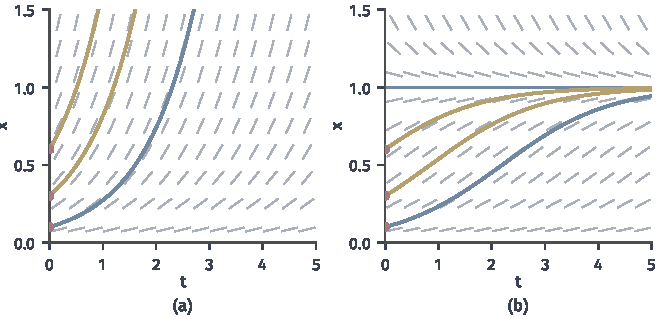
\includegraphics[width=112mm]{figures/06-differential-equations/01-ordinary-differential-equations/matplotlib/ivp-growth-laws/figure.pdf}
 \caption{同一规律、不同初值。灰色短线是方向场，每段的斜率等于右端在该点的值。(a)指数增长$\dot{x}=x$。(b)饱和增长$\dot{x}=x(1-x)$。红点是初值$x_0=0.1,\,0.3,\,0.6$，蓝线是$x_0=0.1$的解，黄线是另两个初值的解。(b)中的水平蓝线$x\equiv 1$也是解。}
 \label{fig:ivp-growth-laws}
\end{BookInlineFigure}

可以把方向场想象成平面上的水流。时间总把水往右推，竖直方向的流速由右端决定。把一片小木片放在初始点上，它漂过的路径就是解曲线。这个比喻说明了两件事：解处处与线段相切，换一个投放点就换一条路径。比喻也有局限：真实的水流中一片木片只走一条路，方程却未必如此，第~\ref{sec:ivp-separable}小节会遇到从同一点分出多条解的例子。

\paragraph{冷却}
第三个例子让规律中出现环境的数据。设$x(t)$是咖啡的温度，室温恒为$c$度。Newton冷却定律假设降温速率与温差成正比，比例系数$k>0$由杯子和空气决定：
\begin{equation}
 \dot{x}=-k(x-c).
 \label{eq:ivp-cooling}
\end{equation}
令$y=x-c$，则$\dot{y}=\dot{x}=-ky$，这是式~\eqref{eq:ivp-exponential}取$r=-k$的情形。由式~\eqref{eq:ivp-exponential-solution}，$y(t)=y_0\mathrm{e}^{-kt}$，换回温度得到
\begin{equation}
 x(t)=c+(x_0-c)\mathrm{e}^{-kt}.
 \label{eq:ivp-cooling-solution}
\end{equation}

取$c=20$，$k=0.1$（每分钟），$x_0=80$。十分钟后温度为$20+60\mathrm{e}^{-1}\approx 42.07$度，此时的变化率是
\[
 \dot{x}(10)=-0.1\times(42.07-20)\approx -2.21,
\]
也就是每分钟下降约$2.21$度。图~\ref{fig:ivp-cooling-field}中紫色线段正是曲线在这一点的切线，它与周围的灰色短线方向一致。

\begin{BookInlineFigure}
 \centering
 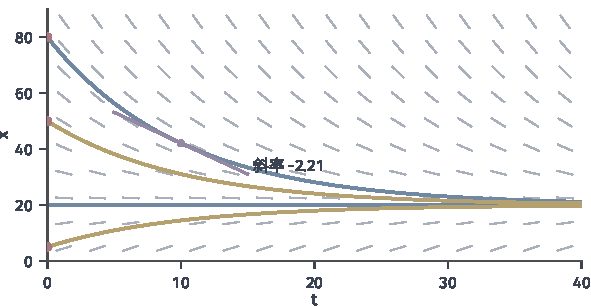
\includegraphics[width=100mm]{figures/06-differential-equations/01-ordinary-differential-equations/matplotlib/ivp-cooling-field/figure.pdf}
 \caption{冷却方程$\dot{x}=-0.1(x-20)$的方向场，时间以分钟计，温度以摄氏度计。蓝线从$80$度出发，黄线从$50$度和$5$度出发，水平蓝线是恒为室温的解。紫色线段是蓝线在$t=10$处的切线，斜率约为$-2.21$。}
 \label{fig:ivp-cooling-field}
\end{BookInlineFigure}

三个例子有共同的结构：一个已知的右端，一个未知的时间函数，一个指定的起点。这里还须说清未知函数定义在哪里，右端在哪里有意义，于是有下面的定义。

\begin{definition}[初值问题]
 \label{def:ivp-ivp}
 设$T\subseteq\mathbb{R}$是区间，$\bm{D}\subseteq\mathbb{R}^{n}$是开集，$\bm{f}:T\times\bm{D}\to\mathbb{R}^{n}$，$t_0\in T$，$\bm{x}_0\in\bm{D}$。\term{初值问题}是寻找一个包含$t_0$的非退化区间$I\subseteq T$，以及曲线$\bm{x}:I\to\bm{D}$，使
 \begin{equation}
 \dot{\bm{x}}(t)=\bm{f}\bigl(t,\bm{x}(t)\bigr),\quad t\in I,\qquad
 \bm{x}(t_0)=\bm{x}_0.
 \label{eq:ivp-ivp}
 \end{equation}
 $t$称为时间，$\bm{x}(t)\in\mathbb{R}^{n}$称为状态，$\bm{f}$称为右端，$t_0$称为初始时刻，$\bm{x}_0$称为\term{初值}（initial value），$I$称为解的\term{存在区间}（interval of existence）。
\end{definition}

“方程成立”的准确含义在第~\ref{sec:ivp-verification}节规定。这个定义中各个对象的地位不同。$\bm{f}$、$t_0$、$\bm{x}_0$、$T$、$\bm{D}$是给定的数据，曲线$\bm{x}$是未知量，存在区间$I$也是答案的一部分，事先并不知道它有多长。式~\eqref{eq:ivp-ivp}的第一式是规律，第二式是起点，缺一不可。标量情形$n=1$时，状态写成不加粗的$x(t)$，右端写成$f(t,x)$，上面的增长与冷却都属于这种情形。

\paragraph{微分方程的分类用语}
含有未知函数导数的等式称为\term{微分方程}（differential equation）。若未知函数只依赖一个自变量，称为\term{常微分方程}（ordinary differential equation，ODE）。方程中出现的最高导数的次数称为\term{阶}（order）。式~\eqref{eq:ivp-exponential}至式~\eqref{eq:ivp-cooling}都是一阶常微分方程。式~\eqref{eq:ivp-ivp}看起来只含一阶导数，下一节会说明高阶方程也能写成这个样子。

\paragraph{初值与两点边值}
初值的特点是所有条件都给在同一时刻。对比一个二阶方程：
\begin{equation}
 \ddot{x}+x=0,
 \label{eq:ivp-harmonic}
\end{equation}
它的解是$x(t)=a\cos t+b\sin t$，其中$a,b$是常数，下面直接代入即可验证：$\ddot{x}=-a\cos t-b\sin t=-x$。两个常数要由两个条件定出来，关键在于条件放在哪里。

若两个条件都放在$t=0$，即给定位置$x(0)=0$和速度$\dot{x}(0)=v$，代入得$a=0$，$b=v$，于是$x(t)=v\sin t$。无论$v$取什么，都恰好得到一条曲线，这就是图~\ref{fig:ivp-ivp-bvp}(a)。

若把条件放在区间的两端，要求$x(0)=0$，$x(\pi)=\beta$，就成了\term{两点边值问题}（two-point boundary value problem）。第一个条件仍给出$a=0$，第二个条件变成
\[
 b\sin\pi=\beta,\qquad\text{即}\qquad 0=\beta.
\]
所以$\beta\neq 0$时一条解也没有，$\beta=0$时每个$b$都给出一条解。图~\ref{fig:ivp-ivp-bvp}(b)中$x(\pi)=1.2$的空心点无法到达，而$x(\pi)=0$的红点被无穷多条曲线同时经过。

\begin{BookInlineFigure}
 \centering
 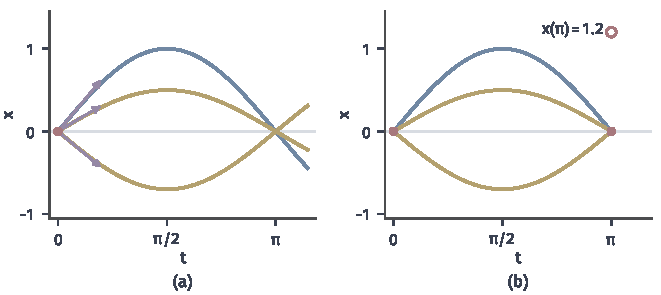
\includegraphics[width=112mm]{figures/06-differential-equations/01-ordinary-differential-equations/matplotlib/ivp-ivp-bvp/figure.pdf}
 \caption{方程$\ddot{x}+x=0$的两种提法。(a)初值问题：$x(0)=0$，紫色箭头表示初速度$v=1,\,0.5,\,-0.7$，每个初速度对应一条解$v\sin t$。(b)两点边值问题：两端红点$x(0)=x(\pi)=0$对应无穷多条解$b\sin t$，图中画出$b=1,\,0.5,\,-0.7$；空心点$x(\pi)=1.2$无解可达。}
 \label{fig:ivp-ivp-bvp}
\end{BookInlineFigure}

差别的根源在于计算的方式。初值问题的全部信息都在起点，可以沿时间一步步往前推。两点边值问题的条件分在两头，必须把整段曲线同时考虑，右端点的要求能否满足，还取决于方程本身。上面$\sin\pi=0$恰好使右端条件失去作用；若把区间长度换成$\pi/2$，条件变成$b=\beta$，解又唯一了。这类问题的一维例子由第~\ref{chap:elliptic-equations}章承接，本部分只讨论初值问题。
